\documentclass[10pt,compsoc]{IEEEtran}
\usepackage[spanish]{babel}
\usepackage{amsmath,amsfonts}
\usepackage{algorithmic}
\usepackage{array}
\usepackage[caption=false,font=normalsize,labelfont=sf,textfont=sf]{subfig}
\usepackage{textcomp}
\usepackage{stfloats}
\usepackage{float}
\usepackage{url}
\usepackage{verbatim}
\usepackage{graphicx}
\hyphenation{op-tical net-works semi-conduc-tor IEEE-Xplore}
\def\BibTeX{{\rm B\kern-.05em{\sc i\kern-.025em b}\kern-.08em
		T\kern-.1667em\lower.7ex\hbox{E}\kern-.125emX}}
\usepackage{balance}
\begin{document}
	\title{El procesador CELL, desde un enfoque
		histórico}
	\author{Ramiro Barcala Roca, Valentin Angrigiani, Gabriel Hackl}
		
	\markboth{Organizacion del Computador, Catedra Marchi, 2024}%
	{How to Use the IEEEtran \LaTeX \ Templates}
	\maketitle
	
	\begin{abstract}
		Este trabajo tratará el procesador CELL de Sony. Se toma un enfoque investigativo y contrastante entre arquitecturas del CELL, y otras de la época (y la actualidad). Las aplicaciones principales para las que fue diseñado, y las aplicaciones que se descubrieron luego, junto  con su importancia histórica. Conceptos básicos de computación heterogénea (distintos nucleos). Analisis a futuro relacionandolo a todo.
	\end{abstract}
	
	\begin{IEEEkeywords}
		SPE,PPE,SIMD,Pipeline-ing, paralelismo, calculos vectoriales, computacion heterogenea, celdas.
	\end{IEEEkeywords}
	
	\section{Introducción}
	\IEEEPARstart{A} mediados de los 2000, mientras los CPU's multinucleo recien se estaban introduciendo al mercado, la empresa Sony empieza a investigar y desarrollar su sistema de entretenimiento "Play-Station 3". Todo esto en un mercado competitivo frente a otras marcas como Microsoft y Nintendo. Terminan diseñando un procesador multi-core, el cual tiene como particularidades los sub-nucleos. Sony tambien quería estandarizar su procesador en dispositivos de todas las gamas y usos multimedias.
	
	Sin embargo, tanto el producto como su procesador,fueron un fracaso comercial. Sin embargo, se descubrieron usos investigativos/científicos/economicos, entre otros.
	
	
	\section{Epoca Pre-CELL}
	\noindent Para ponernos en contexto, vamos a explicar la situacion de las arquitecturas del momento, como de las empresas que lanzaban nuevos productos (del mismo rubro o parecido), en aquella época.
	
	\subsection{Empresas del rubro de las consolas}
	\noindent 
	En el año 2005, las siguientes empresas de consolas/videojuegos, competian en el mercado: 
	\begin{itemize}
		\item{{\bf{Sony}}: parte de un exito rotundo con su anterior producto: la PS2. Tenia grandes expectativas con su nuevo producto, apuesta a lo grande, con nuevas funcionalidades no esenciales (ej: puertos HDMI, Blue-Ray, etc).}
		
		\item{{\bf{Microsoft}}: viene de un exito modesto, con su primer producto: la X-Box. En la X-Box 360, se centra en abaratar su producto, pero proveer servicios en linea de gran calidad. Esto les pasa factura con los problemas de hardware que tendria la consola mas adelante.}
		
		\item{{\bf{Nintendo}}: tuvo un exito pobre en su consola anterior, la Gamecube. En la Wii, se decide no hacer costos de fabricacion muy caros. Pero además, se centra en facilitar experiencias novedosas para el usuario final, mediante el uso de movimientos corporales para controlar los juegos, como extensiones al mismo control (volantes, soportes, etc).}
	\end{itemize}
	
	
	
	Es necesario comprender que la industria de los juegos estaba al auge. No solo se estaba demandando consolas cada vez mas rápidas y potentes, sino también mucha mas gente se introducía a este tipo de consumo.
	

	
	\begin{figure}[H]
	\centering
	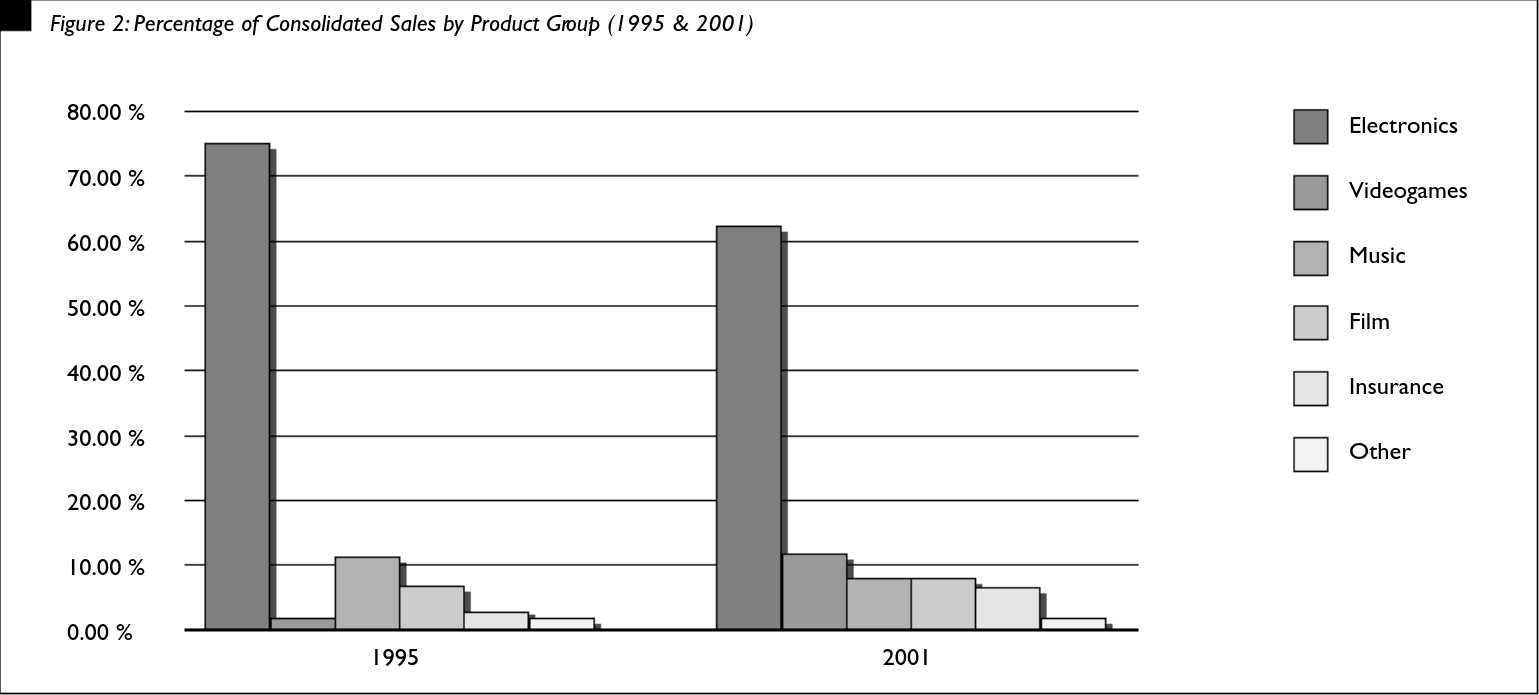
\includegraphics[width=3.5in]{imgs/gamingshare.png}
	\caption{Análisis del mercado del entretenimiento, entrando al nuevo milenio.}
	\label{fig2}
	\end{figure}
	
	

	\begin{figure}[H]
	\centering
	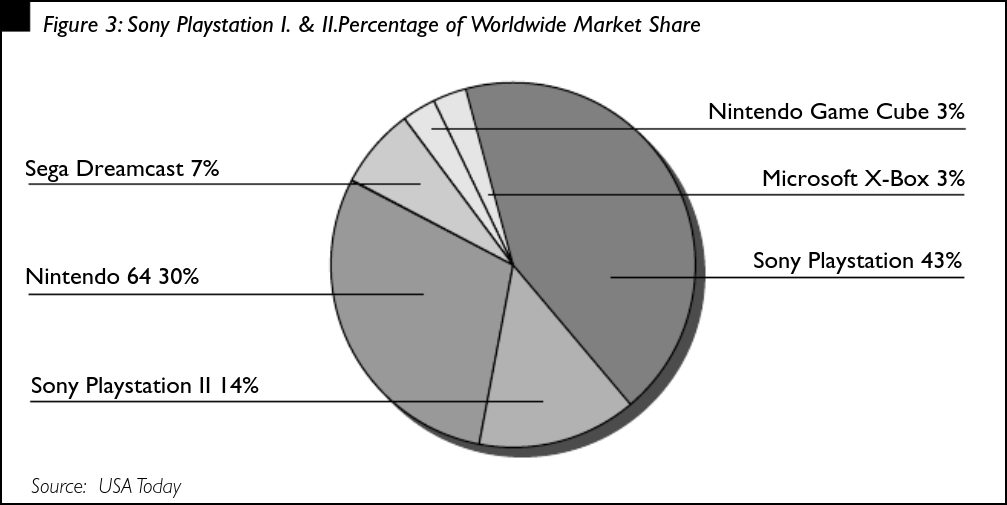
\includegraphics[width=3.5in]{imgs/marketshare.png}
	\caption{Porción del mercado de las consolas, de cada empresa.}
	\label{fig1}
	\end{figure}	
	
	
	\section{Arquitectura CELL}	% MODULOS,ARQUITECTURAS INTERNAS, CONVENCIONES, INSTRUCCIONES, etc
	\noindent Diseñada por Sony, en conjunto con Toshiba e IBM, esta arquitectura trae al mercado un procesador que maneja fuertemente la computación heterogénea, mediante el uso de sus 9 núcleos. 
	
	Si bien originalmente se pensaba incluirlo en dispositivos multimedia y del entretenimiento varios, se termino destinando casi unicamente en la PS3. De todas formas, Sony realmente quería traer una nueva revolución al rubro de diseño de arquitecturas.\newline
	
	\begin{figure}[H]
	\centering
	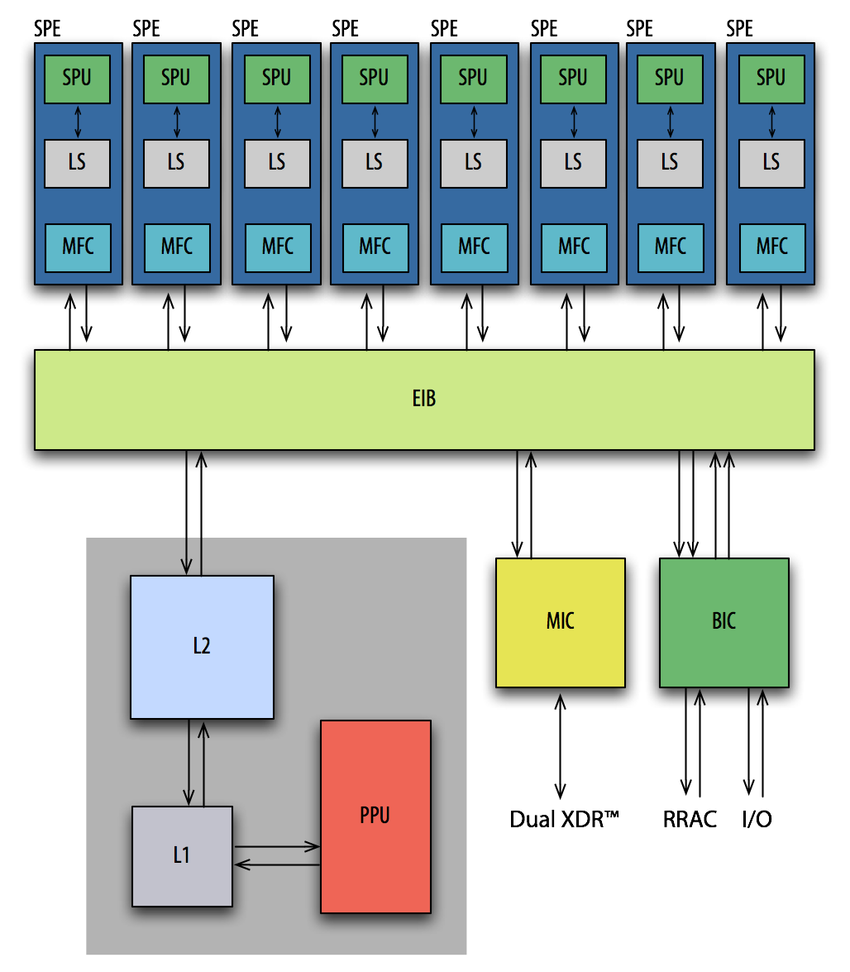
\includegraphics[width=3.5in]{imgs/arquitecturacell.png}
	\caption{Arquitectura del CELL Broadband Engine.}
	\label{fig3}
	\end{figure}
	
	
	\subsection{Distintos módulos del Cell} 
	\noindent Para empezar, hablaremos del PPE (Power Processing Element). Este nucleo, es el principal de la arquitectura. Es de proposito general, y a su vez se encarga de controlar el resto de los sub-nucleos (cargar memoria y ejecutar instrucciones). Estaba conformado por 2 niveles de memoria caché, y un PPU (Power Processing Unit).\newline
	
	Luego, los SPE (Synergistic Processor Element), son los distintos sub-nucleos de la arquitectura. No son de proposito general, mas bien se encargan de realizar operaciones vectoriales, dirigidas desde el PPE. Cada uno tiene su memoria interna (Local Store), y un modulo Memory Flow Controller para poder recibir/transmitir datos desde el Bús, y un SPU (Synergistic Processing Unit).
	Trabajan con instrucciones SIMD con punto flotante, pudiendo llegar a realizar 25,6Gflops por segundo (25,6 mil millones de operaciones de punto flotante/s), por cada SPE. Vale la pena mencionar que las instrucciones SIMD se encargan de aplicar la misma operación a un conjunto de datos, para asi poder obtener un mayor rendimiento en tiempo.\newline
	
	\subsection{Interconexión} 
	\noindent La interconexion de los distintos modulos y nucleos (ademas de la memoria externa, y la interfaz I/O) se realizaba mediante el Element Interconnection Bus. Dicho bus estaba conformado por 4 anillos unidireccionales tokenizados, 2 en cada direcciones. Era un bus tokenizado, por ende la informacion no se retransmitia mas de lo que debia, mediante un identificador del modulo al que debia llegar la informacion. 
	Por como estaba armado, nunca seria posible saturar dicho bus (ancho de banda interno maximo de 204,8GB/s).
	

	
	\subsection{Computacion heterogenea en el Cell }% SIMD
	\noindent La computacion heterogenea puede ser entendida como aquella computacion que requiere el manejo y codificado de instrucciones para una arquitectura que use distintos tipos de nucleos.\newline
	
	A gran escala, podriamos decir que la gran mayoria de consolas o computadoras orientadas al Gaming, hoy en dia, requieren de la misma; Se debe instruccionar al CPU,GPU, etc. Sucede lo mismo con Modelados de Financiacion, o de computacion Cientifica, los cuales se benefician de ambos aspectos. Sin embargo, se puede dar a una escala muchisimo mas chica.\newline
	
	 Resulta que la computacion heterogenea, dentro del Cell, se aplica a los distintos SPE que residen en el mismo. De forma, que no solo programamos el PPE, sino los SPE, los cuales reciben sus instrucciones (y memoria cargada) del anterior mencionado. Ademas, el propio desarrollador puede realizar cierto tipo de pipelining; Paralelizar los programas de los SPE,vectorizandolos y computarizando las salidas de los mismos.\newline
	 
	 El codigo destinado a los SPE's debe ser escrito aparte del programa del PPE, y traducido a codigo maquina por compiladores especificos de SPE's
	
	\subsection{Contraste con arquitecturas actuales}
	\noindent La idea del CellBE era aplicar el tipo de arquitectura de "celdas", donde cada modulo se encarga de una tarea lo mas especifica posible. Así, aplicamos el lema "Divide y vencerás" pudiendo manejar operaciones mas voluminosas y complejas. Tambien, como cada modulo funcionaba por separado, se lo podia escalar tanto como se quisiese. Esto facilito el creado de sistemas que aplicaban este paradigma (como supercomputadoras).\newline
	
	 Mientras que en el CELL se requeria de una computacion heterogenea como la mencionada anteriormente, en las arquitecturas actuales esto no es tan así (no asi en los sistemas que los abarcan. Ej: computadoras dedicadas al Gaming, ya que manejamos nucleos de distintos tipos); las actuales no estan diseñadas con nucleos diferentes, a diferencia del Cell. Entonces, el enfoque al paralelizar tareas variaba; el Cell requeria de un manejo especial por parte del desarrollador (con los SPE's), mientras que hoy en dia hay muchas herramientas que facilitan la division de tareas entre cores.
	
	\subsection{Arquitecturas de la competencia}%ARQUITECTURAS DEL MOMENTO
	\noindent Ya habiendo explicado la arquitectura del CELL, explicaremos algunas de las diferencias con las de la competencia:
	
	\begin{itemize}
				
		\item{{\bf{Microsoft}}: En la X-Box 360, se diseña una arquitectura gracias a IBM que tiene ciertas similaridades con el Cell. Por empezar, el procesador de la consola era el Xenon, de 3 cores. Aquellos cores eran PPE's, como los del Cell, sin embargo, no se encontraba en la arquitectura ningun SPE. Los PPE's, tanto como el resto de modulos, se interconectaban mediante un bús XBAR. A grandes rasgos, es la otra compania del momento la cual tambien busca un acercamiento al paralelismo.}\newline
		
		\item{{\bf{Nintendo}}:En la Wii, tambien se recurre a IBM. Resulta que el procesador que termina ocupando la Wii (Broadway), es un rebranding de la arquitectura ya usada por el producto anterior, la Gamecube. Esto es asi ya que Nintendo pide a IBM un CPU, entonces IBM modifica la arquitectura, haciendola correr a un clock mayor.\newline
		
		Por otro lado, la Wii tambien poseia un Co-Procesador llamado Starlet, el cual se encargaba de tareas menores como el manejo de perifericos o retrocompatibilidad con juegos de consolas anteriores, o hasta del firmware de la consola. Sin embargo, el manejoa de estos dos CPU's se alejaba bastante de la computacion heterogena que requería el Cell.}
	\end{itemize}
	
	\section{Inconveniencias}
	\noindent Debido a que programar los distintos SSP requerían mucho tiempo, una gran cantidad  de desarrolladores pasaron por alto los programas apartes que requerian los mismos, y se centraban unicamente en el PPE, que terminaba realizando todas las tareas. Esto provoca bajos rendimientos en los programas que corria el CELL, ya que sus SPE's quedaban inutilizados.\newline
	
	Muchas tareas que se podian paralelizar, no se estaban ejecutando como debían, ni por los sub-nucleos especializados para eso. Ademas, lo SPE's tampoco tenian branch prediction, por lo que sentencias como if/else eran supervisadas por el PPE, asignandole mas tareas.\newline
	
	 
		
	Esto provoca una performance mediocre en la mayoria de programas realizados por desarrolladores con poco conocimiento y experiencia en este paradigma. El Cell tenia potencial, pero requeria un codigo extremadamente consiso, con pocos condicionales y que mantuviese ocupado a los 7 nucleos totales en todo momento.\newline
	
	Por si no era suficiente, el costo de fabricacion de la consola, durante parte de los primeros 3 años del lanzamiento, rondaba alrededor de los US\$ 900, mientras que el precio para el consumidor final era de US\$ 500; Sumado a que Microsoft ya habia lanzado su consola hace un año atrás, ganando gran parte del mercado. Finalmente los consumidores a los que se destinó el producto, lo rechazan en gran medida.
	
	
	\section{Aplicaciones del CELL}
	\noindent Sin importar el resultado de la aplicacion de la arquitectura, a la arquitectura CELL se la utilizó para otras aplicaciones generales, como modelos de simulacion, o en la computarizacion masiva de datos:
	
	\begin{itemize}
		
		\item{{\bf{Clima}}: Ya que para replicar efectos meteorologicos como las nubes, y para procesar el inmenso volumen de informacion que llega desde los instrumentos usados para las distintas mediciones requería de un sistema que pudiese realizar estas tareas intensivas, se decidió experimentar con esta arquitectura, para diseñar mas adelante una solucion apropiada (que solucionase tambien los problemas que había con el ancho de banda limitado de memoria).}\newline
		
		\item{{\bf{Simulacion}}: Un gran ejemplo de esto es el RoadRunner, una supercomputadora que llegó a operar a 1 petaflops (mill trillones de operaciones de punto flotante/s), capaz de simular explosiones nuclear, y demas cuestiones armamentísticas del gobierno de los Estados Unidos.}\newline
		
		\item{{\bf{Medicina}}: Fue util el cell, ya que facilita procesar la salida de las tomografias computarizadas de un uso intensivo de recursos, para reconstruir imagenes médicas 3D.}

	\end{itemize}
	Como tambien en la industria petrolera y gasífera, en servidores, como tambien en la Construccion y Arquitectura mediante modelos de simulacion.
	
	
	\section{Remanentes del Cell en la Actualidad}%Importancia historica
	\noindent Viendo en retrospectiva, hoy se sigue aplicando hasta cierto punto parte de lo que se promovia en la arquitectura del Cell, pero a gran escala. \newline
	
	Con el diseño de celdas, ejemplos serian las telecomunicaciones, los datos móviles; siendo las distintas celulas las porciones de terreno con cobertura movil, mediante las torres. O tambien como las plataformas funcionando en la nube.	O en los sistemas como computadoras personales, consolas, etc; Tanto en la memoria, diviendose en celdas, o las tareas que realiza un micro-procesador, encargando a los distintos nucleos distintas tareas. Por lo visto, no solo se expandio a arquitecturas, sino a sistemas que abarcan muchas mas cosas.\newline
	
	Este tipo de diseño arquetictural nos permite escalar el sistema con facilidad, pudiendo aumentar la carga de trabajo sin tener que reestructurarlo por completo. Tambien, al suceder fallas, estas se aíslan sobre el modulo erroneo y encapsula el error, para poder modularizar, y reemplazarlos con sencillez. Ademas facilita el paralelismo, enfocando las celdas a propositos simples/unicos y eficientando la utilizacion de recursos.\newline
	
	
	Por otro lado, la computacion heterogenea no se vio tan masificada en el diseño de arquitecturas, pero si en el uso de sistemas que los abarquen. Hoy en dia, interesa mas el poder realizar tareas eficientemente, con arquitecturas especializadas, para despues poder complementarlas en un mismo equipo,no asi como se hacia en CELL, que en la misma arquitectura se encontraban nucleos con propositos distintos. 
		
	\section{Analisis a futuro}
	\noindent Habiendo visto las distintas aplicaciones que hay hoy en dia con las arquitecturas basadas en celdas, creemos que seguira al alza. No solo se seguirá aplicando a los diseños de microprocesadores y sistemas, sino que se expandira a muchos de los rubros en los que hoy no se lo toma en cuenta. \newline
	
	Un ejemplo seria en la agricultura, dividiendo en parcelas los cultivos o ganados, y controlando las cosechas o animales, para revisar en cual se debe focalizar una atención especial. O tambien en los hospitales, buscando aquellos pacientes que requieran un cuidado particular.\newline
	
	Ahora, creemos que la computacion heterogenea si tiene lugar en el futuro, pero algo similar a como pasa en la actualidad. No que se centre en el interior de los distintos diseños minimales, sino de la manera mas abstracta posible.
	
	
	\section{Conclusion}
	\noindent Creemos que, si bien el enfoque que tomo Sony con su arquitectura originalmente compartida por dispositivos varios del mundo del entretenimiento no tuvo un exito considerable, fue util para aproximarse al mundo de la computacion heterogenea, y para darle otro foco a la capacidad de conseguir un mayor rendimiento en los procesadores venideros, no solo aumentando el clock de los mismos.\newline
	
	Ademas, tuvo bastante importancia su experimento con las arquitecturas basadas en celdas, ya que le permitio a las distintas industrias que hoy lo aplican, ver sus beneficios.
	
	
		\begin{thebibliography}{1}
			
			\bibitem{ams}
			{\it{Laboratorio de Arquitecturas Avanzadas con Cell y PlayStation 3}}, Universitat de València, por Fernando Pardo y Jose A. Boluda.\newline
			
			\bibitem{ams}
			{\it{The PlayStation 3 for High Performance Scientific Computing}}, University of Tennessee: Jakub Kurzak, Alfredo Buttari, Piotr Luszczek, Jack Dongarra\newline
			
			\bibitem{ams}
			{\it{The impact of IBM Cell technology on the programming paradigm in the context of computer systems	for climate and weather	models}}, Shujia Zhou, Daniel Duffy, Thomas Clune, Max Suarez, 	Samuel Williams, Milton Halem.\newline
			
			\bibitem{ams}
			{\it{Architecture of Consoles: A practical analysis by Rodrigo Copetti}}, 
			https://www.copetti.org/writings/consoles/\newline
			
			\bibitem{ams}
			{\it{Cell Technology Tackles 3D Medical Imaging Reconstruction Challenges}}, https://www.techbriefs.com/component/content/article/6088-10976-400\newline
			
			\bibitem{ams}
			{\it{Breaking the petaflop barrier}},
			https://www.ibm.com/history/petaflop-barrier\newline
			
			\bibitem{ams}
			{\it{Introducing the IBM/Sony/Toshiba Cell Processor ? Part I: the SIMD processing units}},
			https://arstechnica.com/features/2005/02/cell-1/\newline
			
			\bibitem{ams}
			{\it{The PlayStation Supercomputer}},
			
			 https://www.datacenterdynamics.com/en/analysis/the-playstation-supercomputer/\newline
	
			\bibitem{ams}
			{\it{Console wars: A rare bright spot in the gloomy technology industry, video games are growing up}}, 
			https://www.economist.com/business/2002/06/20/console-wars\newline
			

			\bibitem{ams}
			{\it{Console wars}},
					
			https://www.gainesville.com/story/news/2006/11/11/waging-console-war/31502430007/\newline
			
			\bibitem{ams}
			{\it{PlayStation 3, Console Wars and the Costs of Complexity}},		
			https://techliberation.com/2006/09/07/playstation-3-console-wars-the-costs-of-complexity/\newline
			
			
			\bibitem{ams}
			{\it{PlayStation 3, Console Wars and the Costs of Complexity}}, 			
			https://arstechnica.com/features/2005/02/cell-1/\newline
			
			\bibitem{ams}
			{\it{Cell-Based Architecture: The Backbone of Scalable Systems}}, 			
			https://medium.com/@jishanrandika/cell-based-architecture-the-backbone-of-scalable-systems-2b5ea50cbe1c
			
		
		\end{thebibliography}
		
			
	
		
\end{document}
